After testing analog sorting on a prototype analog computer chip and simulating the process using an ODE solver, we can evaluate its time and space complexity. 

Compared to the other sorting algorithms mentioned at the beginning of the paper, analog sorting performs better in terms of time complexity. However, due to the nature of circuits, it is not as space efficient as most other popular sorting algorithms.

\subsection{Functionality validation of analog sorting}

\begin{figure}[h]
\centering
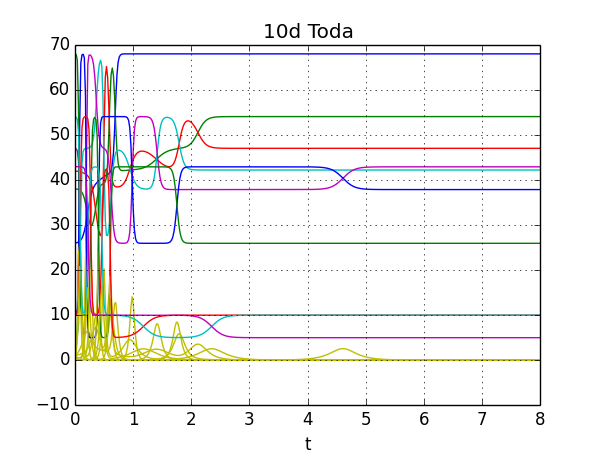
\includegraphics[width=\columnwidth]{graphics/10d_toda_7.png}
\caption{Simulated sorting a 10 element vector.}
\end{figure}

We see in Figure 1, generated from the ODE solver, that the sorting system has periods of swapping, interspersed in quiet periods of little change. The ODE solver was used on a 10 element vector. 

The output of the analog chip, run on two variables and over multiple loops, is shown in the below image.

\begin{figure}[h]
\centering
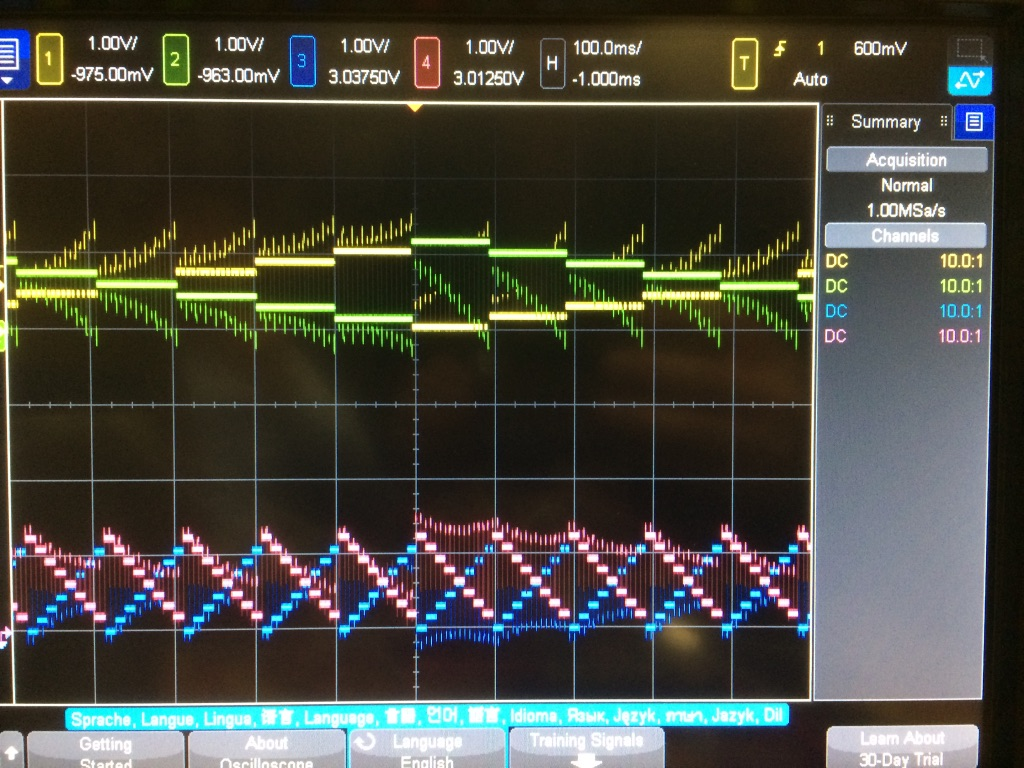
\includegraphics[width=\columnwidth]{graphics/2d_analog.jpg}
\caption{Sorted 2 elements using analog computer chip.}
\end{figure}

 

\subsection{Time cost of the discrete QR algorithm}
Time cost of overall QR loop:
	how many iterations of qr til convergence?
	% time to convergence of qr w.r.t.. problem size
	Since we know the ODE is analogous to QR algorithm, they should take the same amount of time.
Time cost of QR step:
	Numerical Recipes 3rd Edition p585 says the QR algorithm takes $O(N)$ time for symmetric tridiagonal matrices.

\subsection{Time cost of analog sorting}

In terms of time, the sorter takes at least $O(N)$ time because of the time it takes just for signals to propagate across the circuit.
Another issue is the time it takes for the ODE to settle to its final value.
This shows preliminary data showing the time to convergence of analog sorting, plotted against problem size.

\begin{figure}[h]
\centering
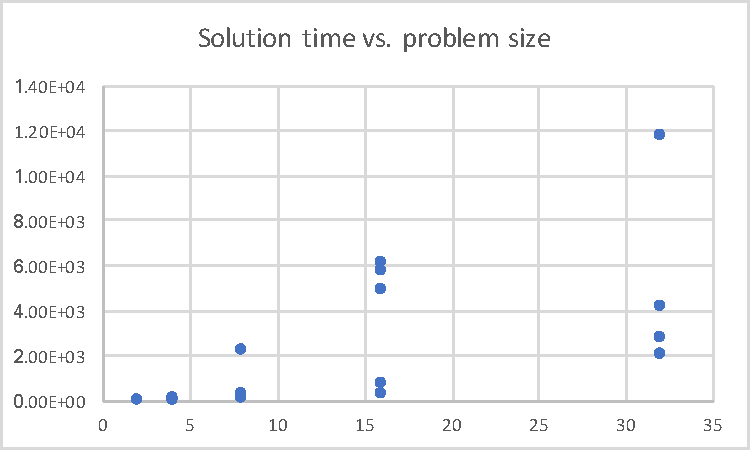
\includegraphics[width=\columnwidth]{graphics/ode_time_vs_problem_size.pdf}
\caption{Preliminary time to convergence vs. problem size.}
\end{figure}

The axes are the time to solution, plotted against $N$, the number of real numbers we are sorting.
The data points come from multiple random trials at each $N$.
The set of real numbers is randomly generated from a chosen dynamic range.
It appears that as the $N$ size increases, the average time grows linearly with respect to $N$.
Furthermore, the variance of the solution time, measured as the standard deviation, also grows.

\begin{figure}[h]
\centering
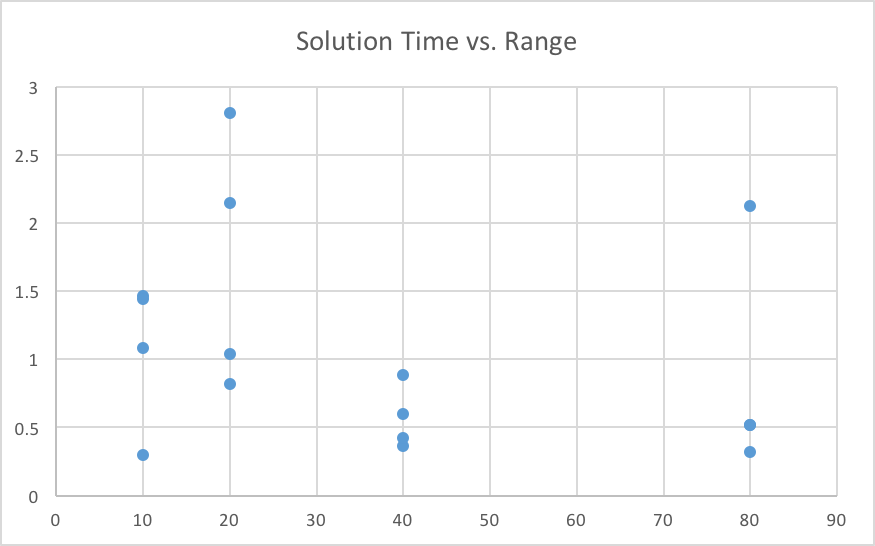
\includegraphics[width=\columnwidth]{graphics/range_vs_solution.png}
\caption{Preliminary time to convergence vs. dynamic range.}
\end{figure}

Another possible factor for solution time to consider is the dynamic range of the real numbers to sort. However, running the simulation on a constant number of elements with different dynamic ranges did not show any significant trends.

\subsection{Hardware cost of analog sorting}

Analog sorting on the chip relies on the hardware components needed to build the circuit. 
We need a constant amount of components for each of the $N$ ODEs.
Thus, the analog sorter takes up $O(N)$ amount of circuit components to sort $N$ elements.

\subsection{Limitations}

As mentioned before, the choice of initial $y$ values affects the sorting mechanism. Changing the initial values of the off-diagonals impacts whether or not the algorithm ever reaches a correctly sorted state of the diagonal entries.

Setting the initial values for the off-diagonals to $0$ will prevent the algorithm from starting in the first place. Initial $y$ values that are too small may stop the algorithm mid-way and result in an approximate sorting with two elements being out of place. After the diagonal entries converge to their final state, the $y$ values are nonzero, but in the magnitude of less than $10^{30}$. How big the initial off-diagonal entries have to be might depend on the range of the numbers to sort.

Brockett mentions briefly that $H_\infty$ will be sorted in almost all cases, but does not elaborate on the exceptions ~\cite{brockett}.


% \begin{figure}
% \centering
% \includegraphics[height=1in, width=1in]{fly}
% \caption{A sample black and white graphic
% that has been resized with the \texttt{includegraphics} command.}
% \end{figure}

% \begin{figure*}
% \centering
% \includegraphics{flies}
% \caption{A sample black and white graphic
% that needs to span two columns of text.}
% \end{figure*}

% \begin{figure}
% \centering
% \includegraphics[height=1in, width=1in]{rosette}
% \caption{A sample black and white graphic that has
% been resized with the \texttt{includegraphics} command.}
% \vskip -6pt
% \end{figure}